\graphicspath{{chapters/05_results/images}}
\chapter{Results}

% The Results part describes all the experiments performed and their statistical analysis (at least 10, maximum 40 pages). If you want to provide replication data, include them in another appendix (Appendix II).

\section{Pixel preprocessing statistics}

\subsection{Expected counts computation}

In order to normalize for genomic distance, it is necessary to compute some summary statistic for the pixels at a certain genomic distance; here we compare the statistics obtained using cooltools and HiCONA. 

It is known that the probability of two genomic regions interacting by chance decays exponentially with their distance from each other; for this reason, we expect the function describing probability of contact given distance to be linear in a log-log plot. This is exactly what it is observed in the left panel of image \ref{fig:cooltools}.

When processing a file with a specific set of filtering parameters, one curve is computed for each individual chromosome. This is done to avoid relying on the assumption that random contact probability decays at the same rate in all chromosomes. One might argue that considering all pixels jointly would yield a more robust and less noisy curve; while that would indeed be the case, each chromosome has enough pixels to obtain a robust curve on its own (aside from chromsome Y).

The image on the left 



% Plot of Hicona expected count vs cooltool ones
\begin{figure}[h]
  \centering
  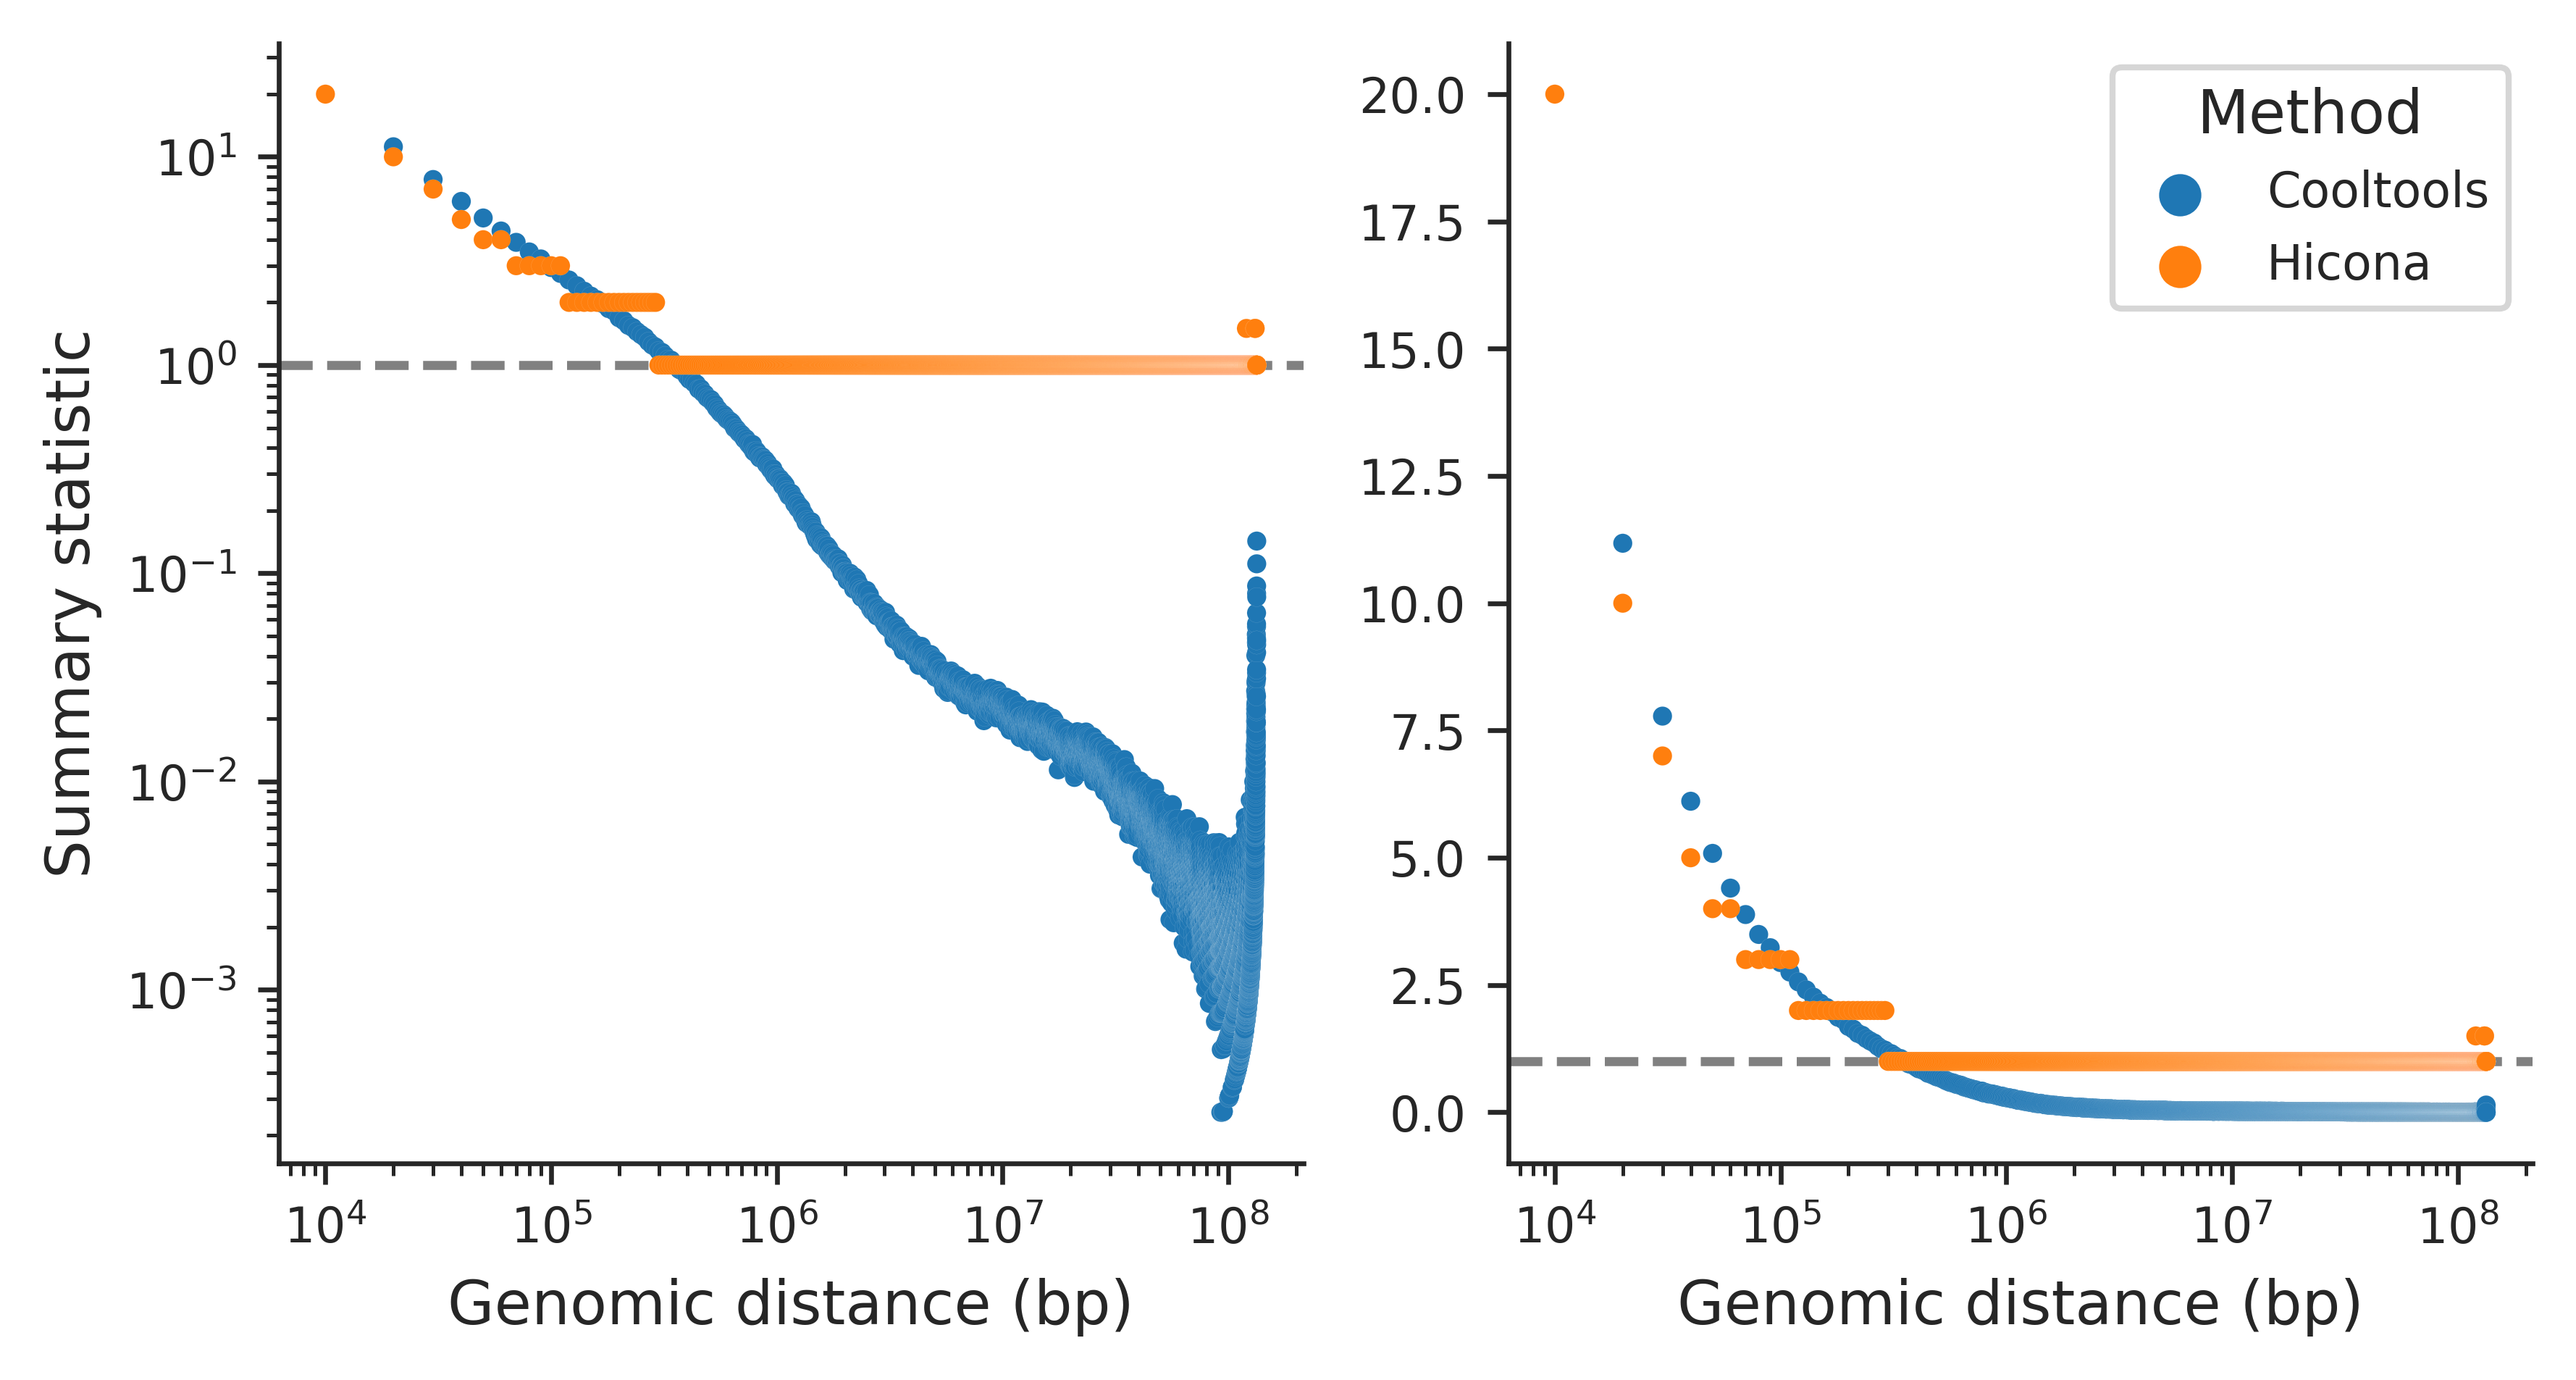
\includegraphics[width=1\textwidth]{hicona_vs_cooltools.png}
  \caption{\textbf{Comparison of summary statiscs from HiCONA and cooltools}. Comparison of the genomic distance normalization factors for chromosome 1 of IMR90 cells, filtered using 200 Mb as genomic distance threshold, obtained using HiCONA and cooltools (for the exact formulas see the Matherials and Methods section). On the left, normalization factor with respect to distance in log-log scale, on the right same plot but without log-transform of the y-axis.}
  \label{fig:cooltools}
\end{figure}


\subsection{Pixels normalization}
% Plot from first lab meeting with distribution prior and after normalization

\begin{figure}[h]
  \centering
  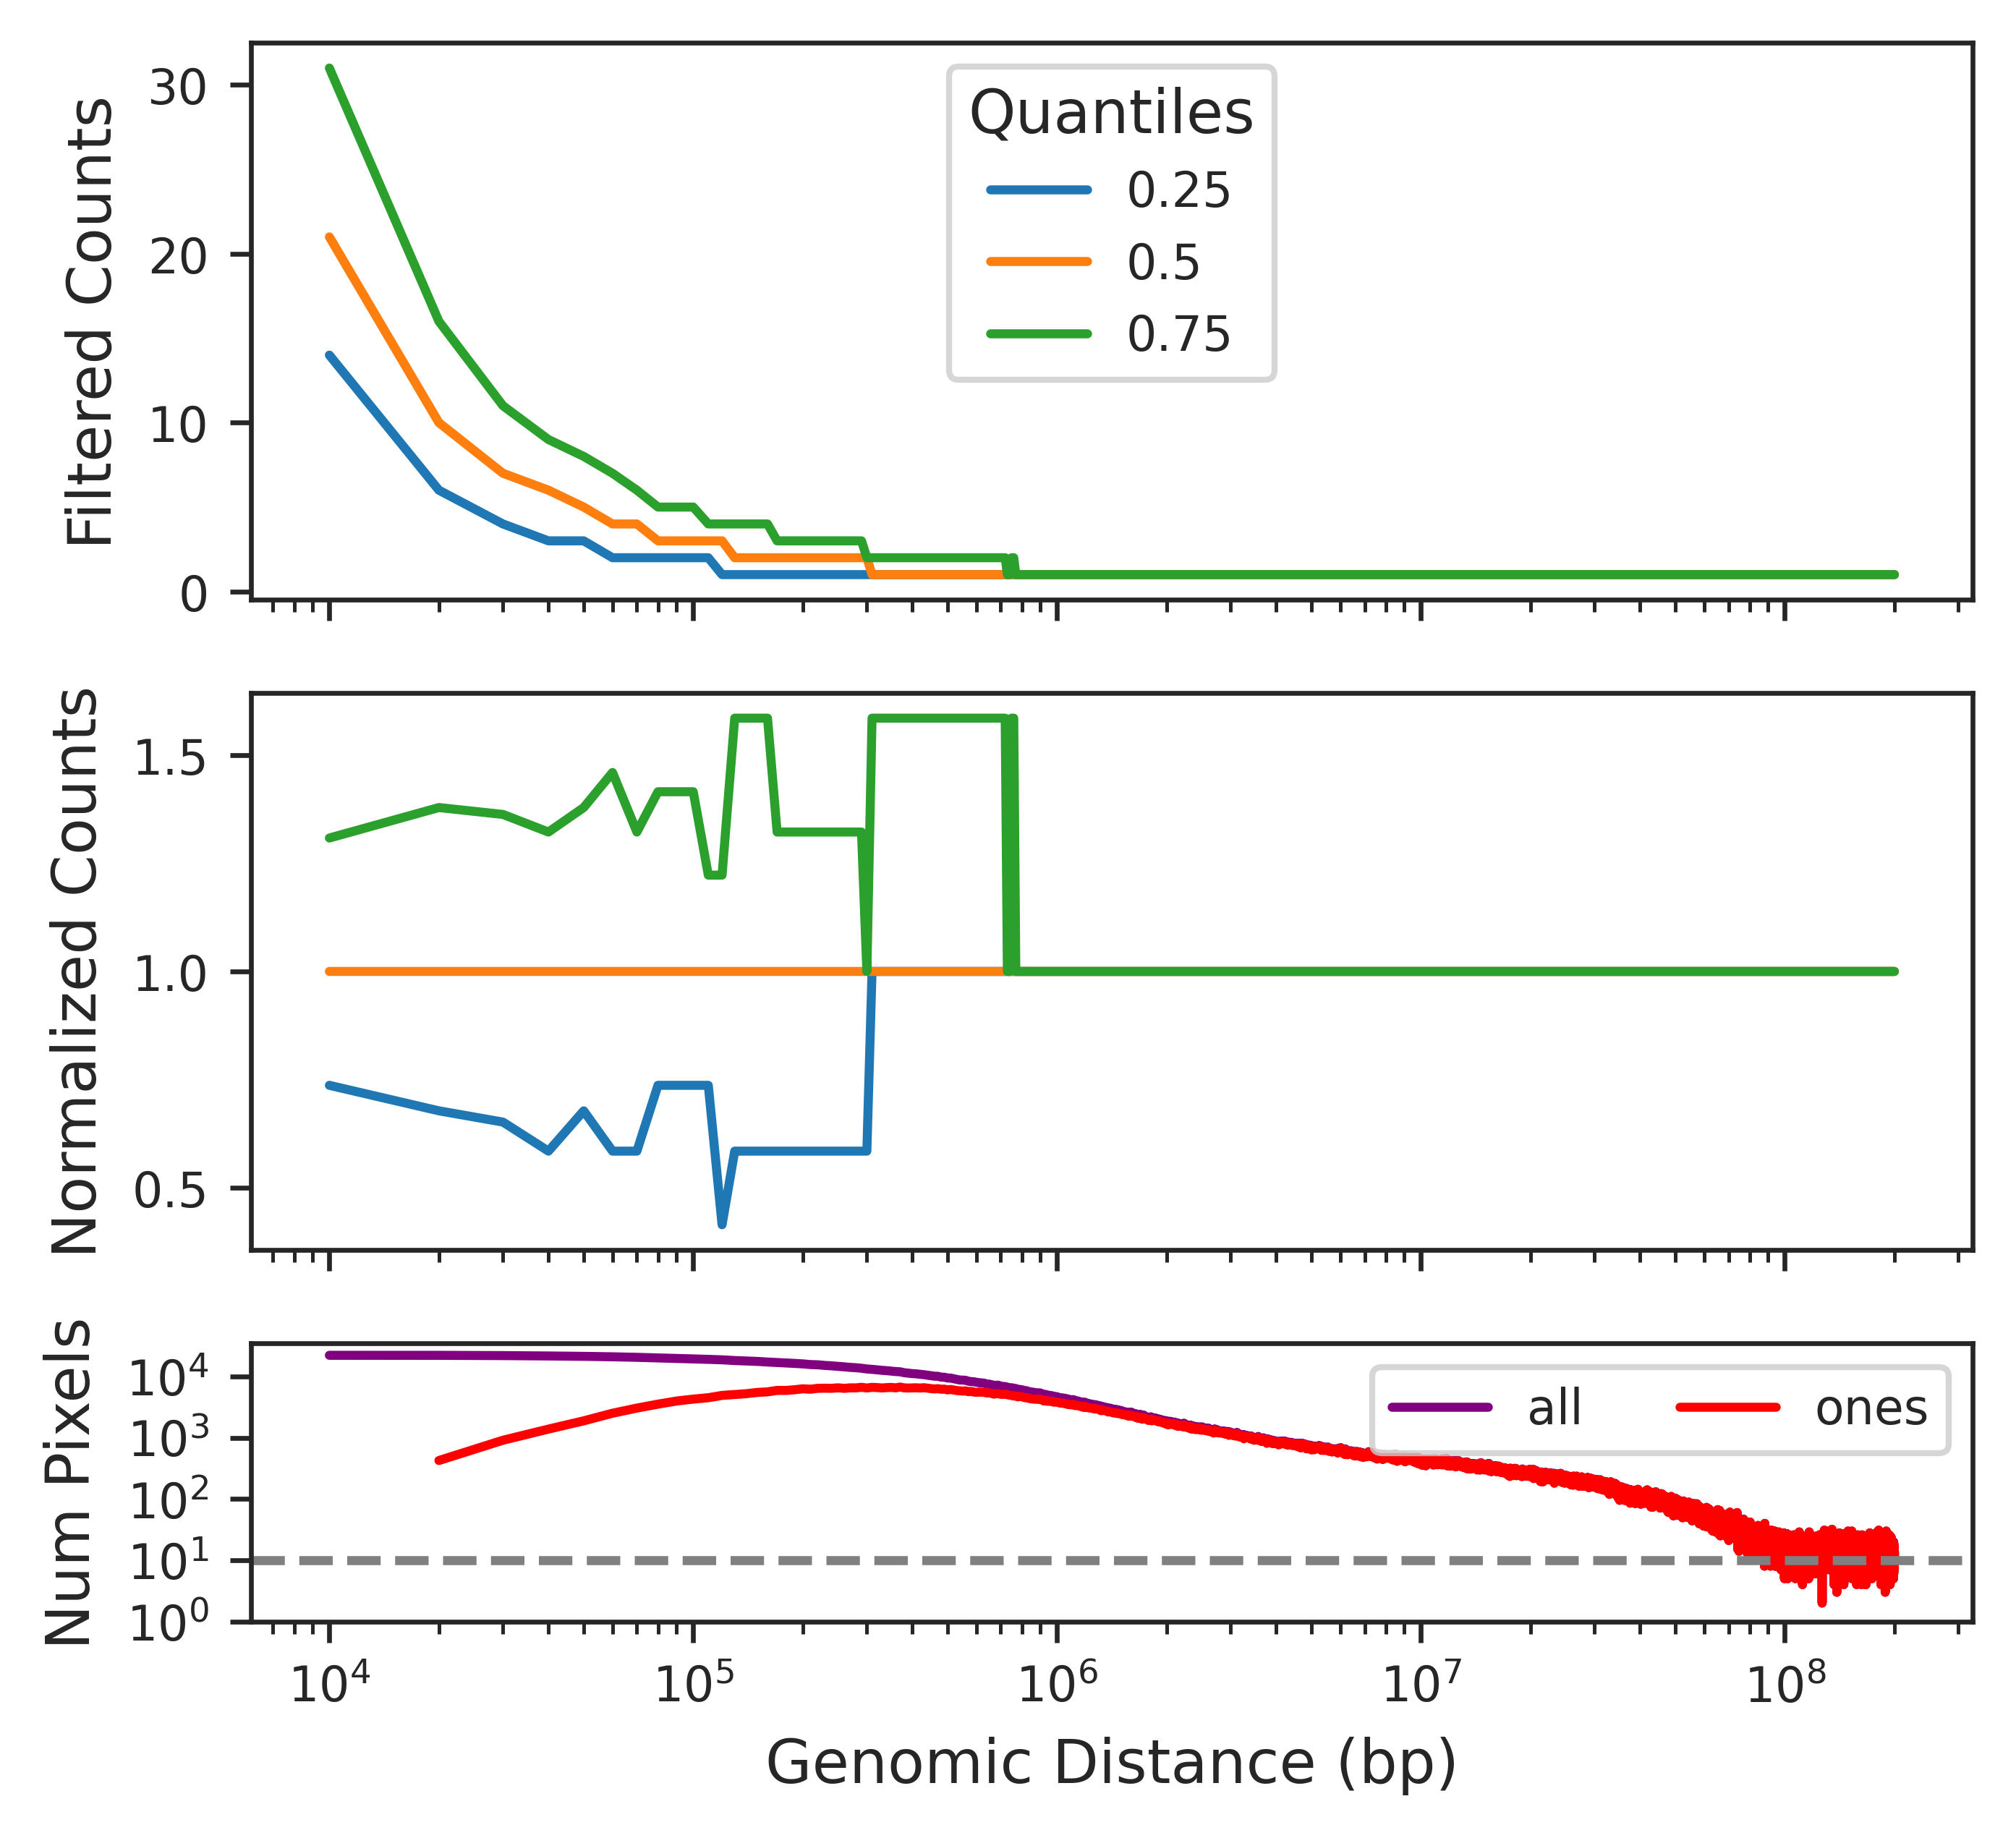
\includegraphics[width=1\textwidth]{normalization_stats.png}
  \caption{\textbf{LIPSUM}. LIPSUM}
  \label{fig:normstats}
\end{figure}

\subsection{Optimal alpha computation}
% Plot alpha computation grid for some file (maybe multiple sets of params)

\begin{figure}[h]
  \centering
  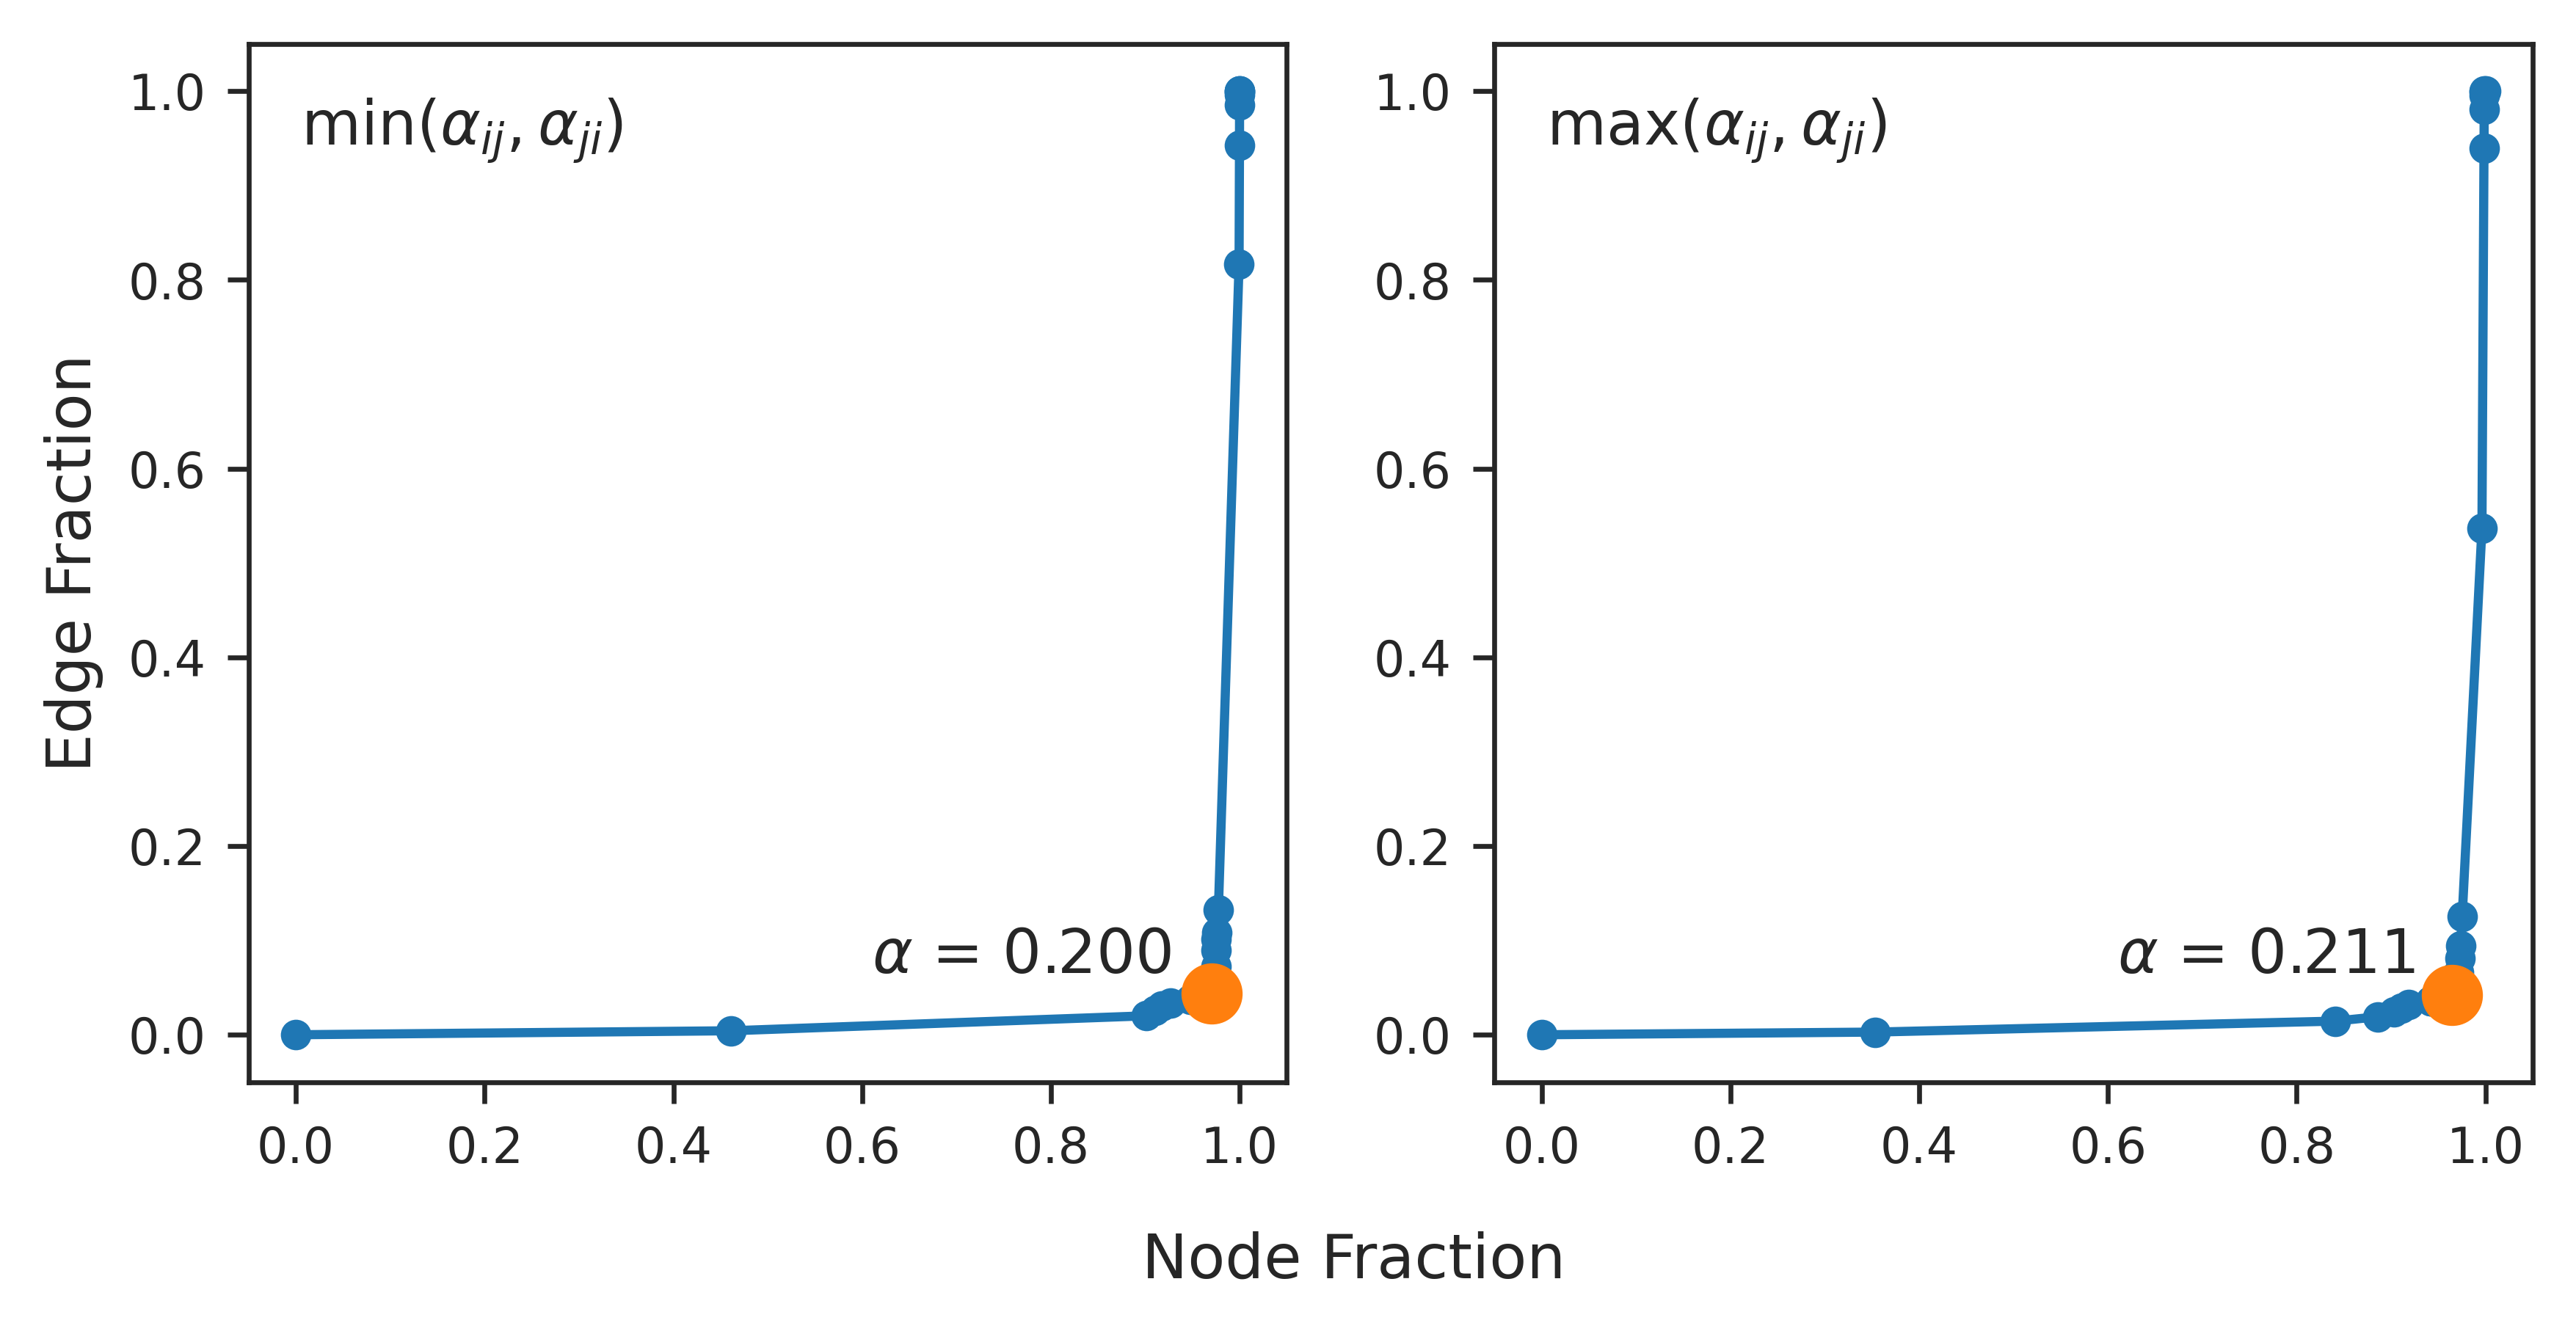
\includegraphics[width=1\textwidth]{alpha_tables.png}
  \caption{\textbf{Optimal alpha selection process}. To define the optimal alpha value to sparsify the chromosome-level network, local search is performed. On the left, set of points tested while trying to find the optimal alpha value for chromosome 1 of IMR90 cells, sparsified using... }
  \label{fig:alphas}
\end{figure}


\subsection{Retained pixels}

\begin{figure}[h]
  \centering
  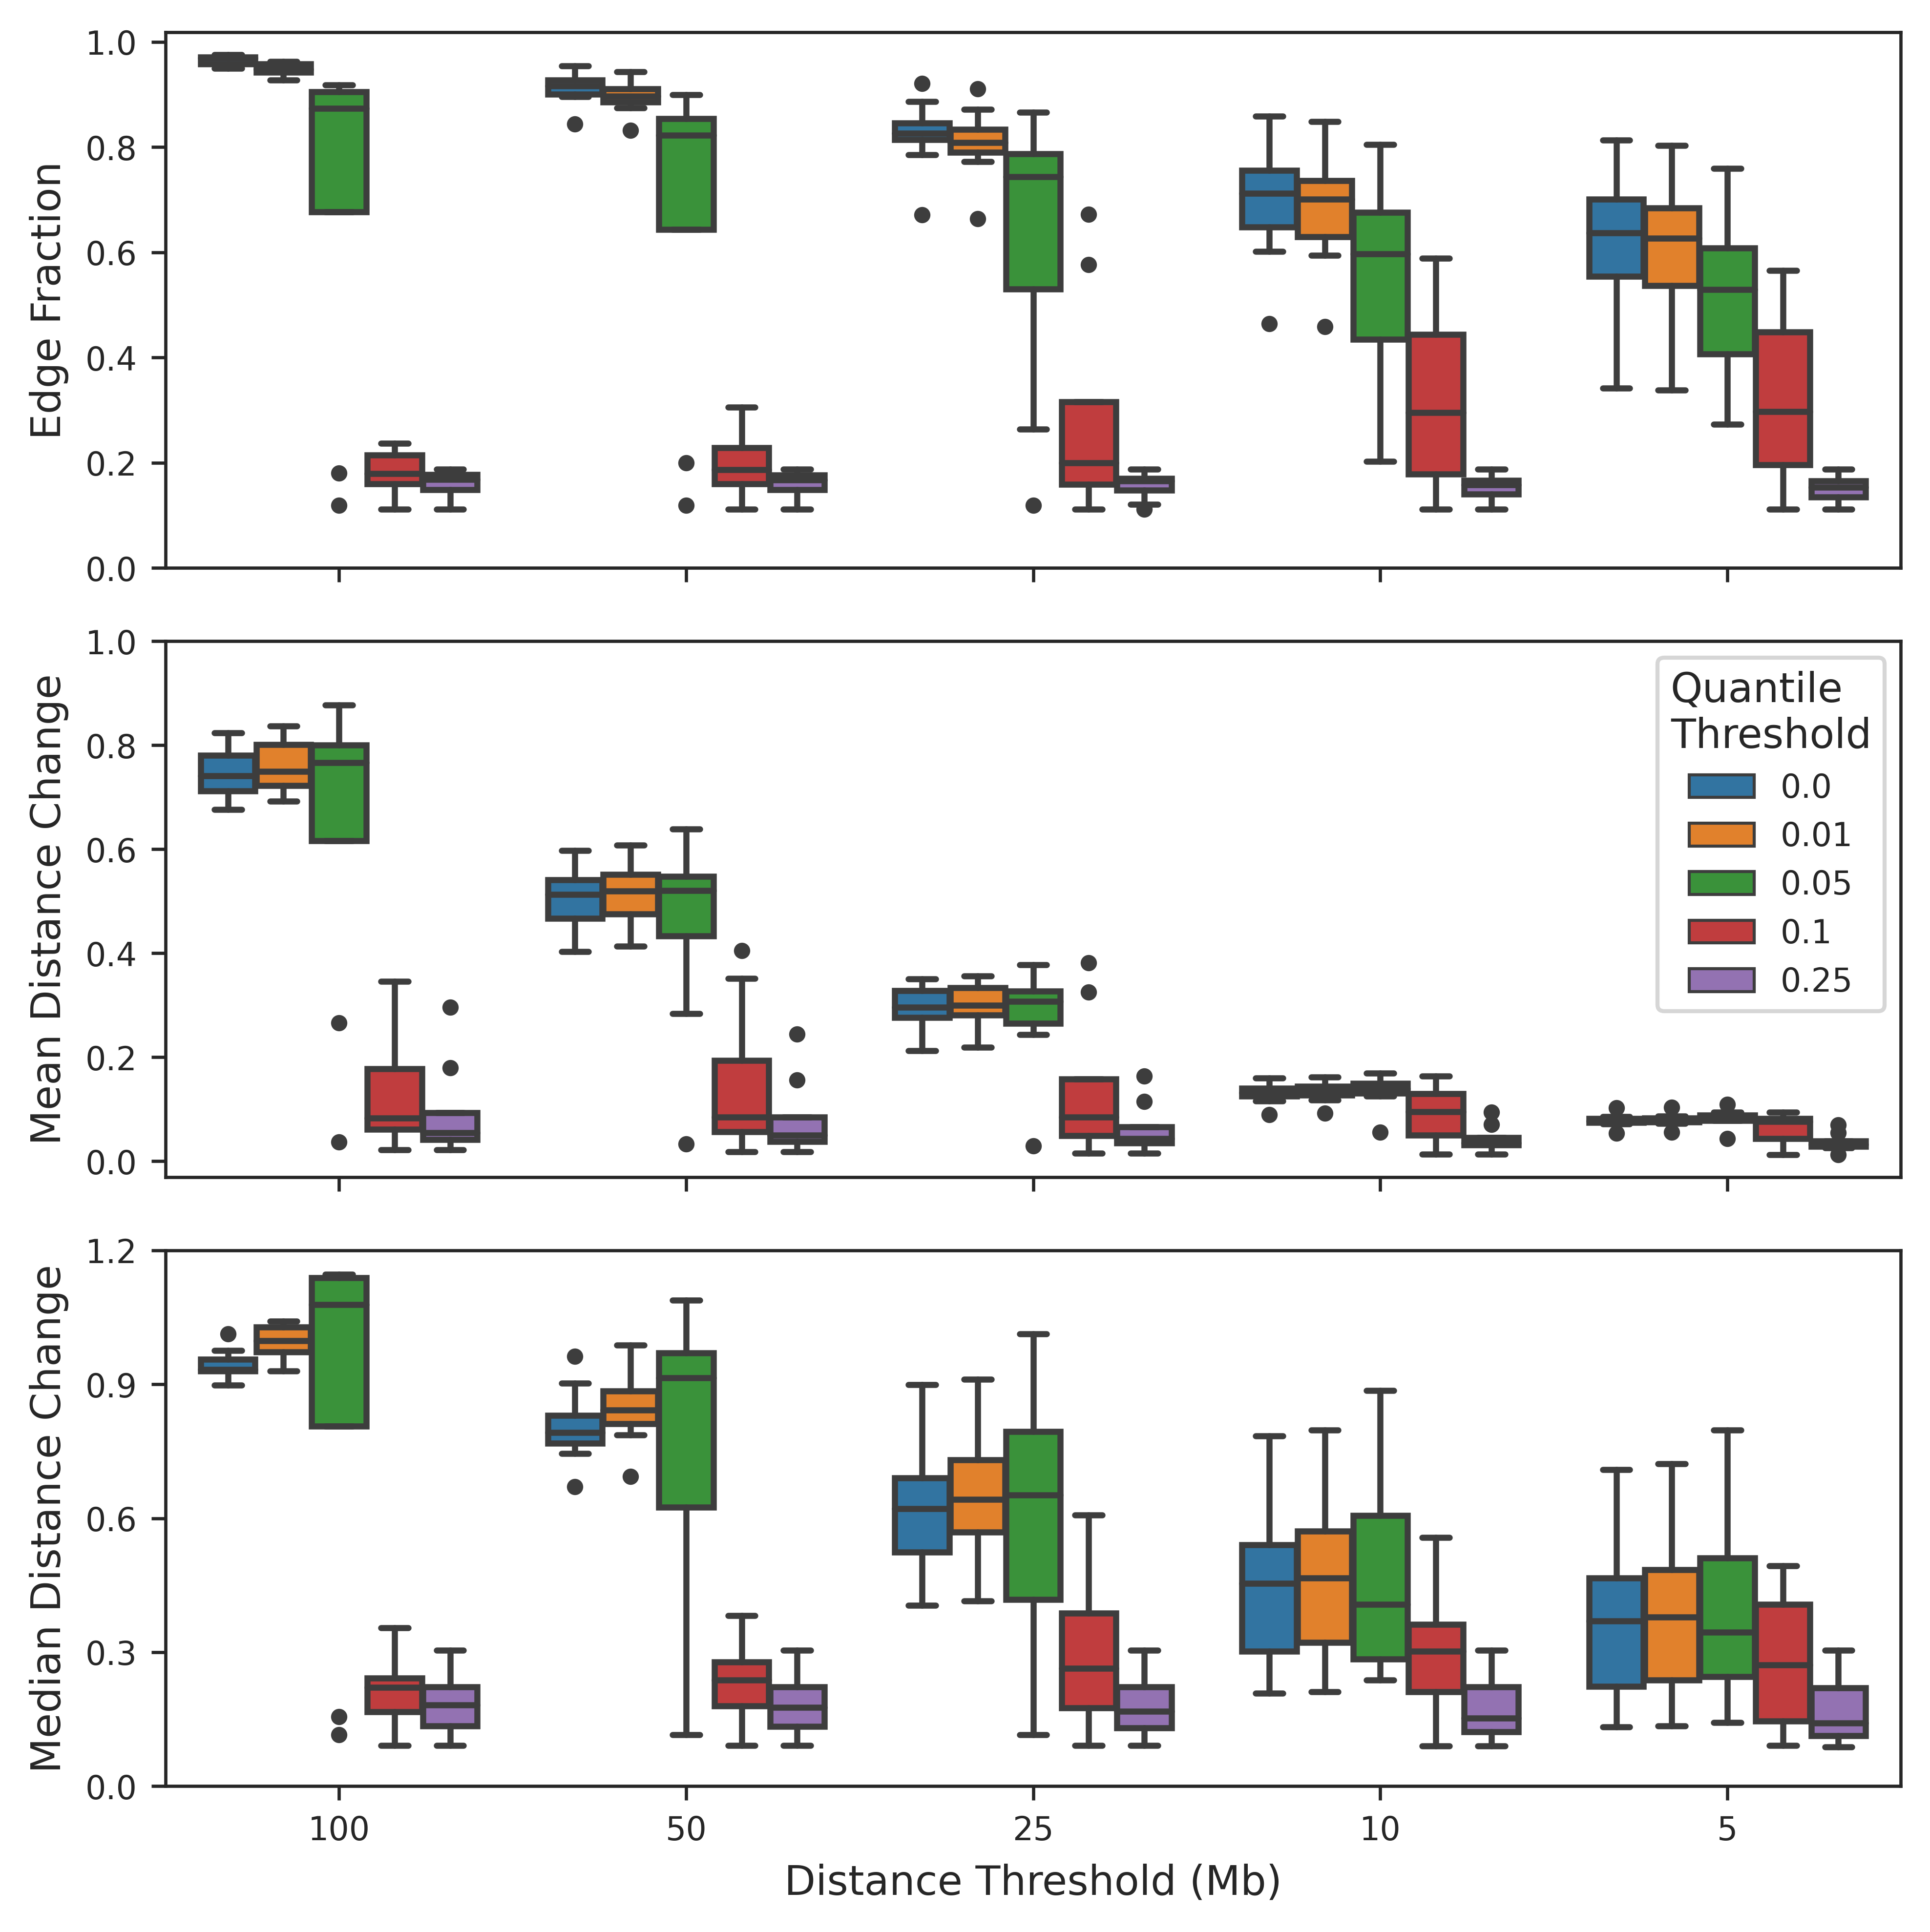
\includegraphics[width=1\textwidth]{filtering_stats.png}
  \caption{\textbf{LIPSUM}. LIPSUM}
  \label{fig:filtering}
\end{figure}

% Plot number of pixels as function of parameters
% Plot variation coefficient with other tools too
\subsection{Expected distance}
% Plot distance of pixels as function of parameters
% Plot expected interaction distance with respect to other tools
\subsection{Consistency on replicates}
% Plot Jaccard index on replicates 
% Plot Jaccard index vs file size pre and after processing
% Plot Jaccard index with respect to other tools

\section{Pixel preprocessing performance}

\subsection{Time benchmark}
% Plot number of filtered pixels vs time (linear)
\subsection{Memory benchmark}
% Plot of the run of a single file using memprof

\section{Pixel preprocessing validation}

\subsection{Pixel annotation enrichment}
% Plot edge annotation fraction
% Plot edge annotation enrichment

\section{Network analysis}

\subsection{Node-label permutations}
% Plot node-label permutation for 1 file, chromosome-wise (maybe new ann)



% ? Plot Hi-C maps at different steps
% TODO: Maybe use in memory benchmarking
% It follows that the reported file size is then 20 bytes times the number of rows of the pixel table. Since two columns of the pixel table ("bin1\_id" and "bin2\_id") are vectors of 64-bit signed integers, while the remaining one ("count") is a vector of 32-bit signed integers, each row of the pixel table requires 20 bytes of memory.